
%%% Local Variables:
%%% mode: latex
%%% TeX-master: "../os-book-pt_BR"
%%% End:

\def\shift{2cm}
\begin{figure}
\centering
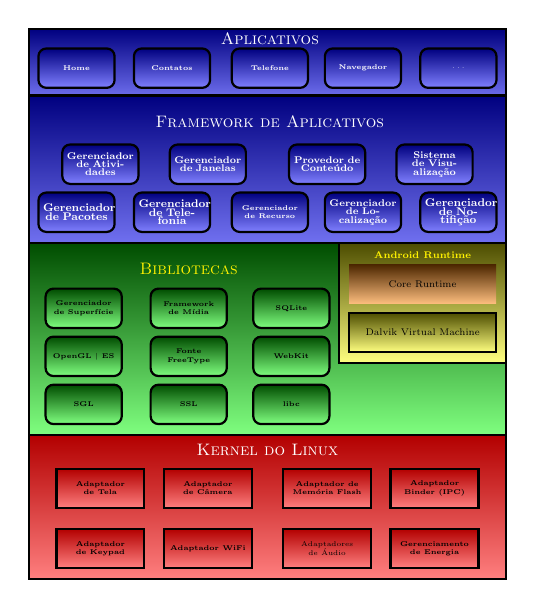
\begin{tikzpicture}
[thick,
global scale/.style={
                scale=#1,
                every node/.style={scale=#1}},
scale=.5,
every node/.style={
  font=\bf\tiny,transform shape
},
app/.style={
  top color=blue!50!black, middle color=blue, bottom
  color=blue!50!white,text=white, minimum height=.5*\shift,  
  text width=.85*\shift, text centered, minimum width=.125*\textwidth,draw
},
lib/.style={
  top color=green!30!black, middle color=green, bottom
  color=green!50!white,text=black,minimum height=.5*\shift,  
  text width=.85*\shift, text centered,draw
}, 
runtime/.style={
  top color=yellow!30!black, middle color=yellow, bottom
  color=yellow!50!white,text=white, minimum height=.5*\shift,  
  text width=\shift, text centered, font=\scriptsize, draw
}, 
corelib/.style={
  top color=orange!30!black, middle color=orange, bottom
  color=orange!50!white,text=white, minimum height=.5*\shift,  
  text width=\shift, text centered, font=\scriptsize
}, 
kernel/.style={
  top color=red!70!black, middle color=red, bottom
  color=red!50!white,text=black, minimum height=.5*\shift,  
  text width=\shift, text centered,draw
}, 
module/.style={
  minimum width=\textwidth, minimum height=\shift,draw
},
component/.style={
  rounded corners=1mm
},
modulelabel/.style={
  color=white, font=\large\sc
},
thebackground/.style={minimum width=\textwidth}
]

% Applications
\node[app,module] (applications) at (0,0) {};
\node[component, app] at (-.4\textwidth,0) {Home};
\node[component, app] at (-.2\textwidth,0) {Contatos};
\node[component, app] (phone) at (.005\textwidth,0) {Telefone};
\node[component, app] at (.2\textwidth,0) {Navegador};
\node[component, app] at (.4\textwidth,0) {$\ldots$};
\node [modulelabel, above of=phone, yshift=-.125*\shift] {Aplicativos};  

% Application Framework
\def\yshift{1.2\shift}
\node[app,module,minimum height=3.5*\yshift] (framework) [below of=applications, yshift=-1.5*\yshift] {};
% 1st layer
\node[component, app] at (-.35\textwidth,-2*\yshift) {\scriptsize Gerenciador de Atividades};
\node[component, app] at (-.125\textwidth,-2*\yshift) {\scriptsize Gerenciador de Janelas};
\node[component, app] at (.125\textwidth,-2*\yshift) {\scriptsize Provedor de Conte\'udo};
\node[component, app] at (.35\textwidth,-2*\yshift) {\scriptsize Sistema de Visualiza\c{c}\~ao};
% 2nd layer
\node[component, app] at (-.4\textwidth,-3*\yshift) {\footnotesize Gerenciador de Pacotes};
\node[component, app] at (-.2\textwidth,-3*\yshift) {\footnotesize Gerenciador de Telefonia};
\node[component, app] (resource) at (.005\textwidth,-3*\yshift) {Gerenciador de Recurso};
\node[component, app] at (.2\textwidth,-3*\yshift) {\scriptsize Gerenciador de Localiza\c{c}\~ao};
\node[component, app] at (.4\textwidth,-3*\yshift) {\footnotesize Gerenciador de Notifi\c{c}\~ao};
\node [modulelabel, above of=resource, yshift=.65*\shift] {Framework
  de Aplicativos};  

% LIBRARIES
\node[lib,module,minimum height=4*\yshift,thebackground] [below of=framework, yshift=-2.5*\yshift] {};
% 1st layer
\node[component, lib] at (-.385\textwidth,-5*\yshift) {Gerenciador de Superfície};
\node[component, lib] at (-.385\textwidth,-6*\yshift) {OpenGL $|$ ES};
\node[component, lib] at (-.385\textwidth,-7*\yshift) {SGL};
% 2nd layer
\node[component, lib] (midia framework) at (-.165\textwidth,-5*\yshift) {Framework de M\'idia};
\node[component, lib] at (-.165\textwidth,-6*\yshift) {Fonte FreeType};
\node[component, lib] at (-.165\textwidth,-7*\yshift) {SSL};
% 3rd layer
\node[component, lib] at (.05\textwidth,-5*\yshift) {SQLite};
\node[component, lib] at (.05\textwidth,-6*\yshift) {WebKit};
\node[component, lib] at (.05\textwidth,-7*\yshift) {libc};
% libraries label
\node [yellow,above of=midia framework] {\sc\large Bibliotecas};


% ANDROID RUNTIME
\node[runtime,module,minimum width=.35\textwidth, minimum
height=2.5*\yshift] (runtime) [below of=framework, yshift=-1.75*\yshift,xshift=.325\textwidth] {};
\node[corelib,text width=3.5cm,fill=blue,text=black] (core runtime) at (.325\textwidth,-4.5*\yshift) {Core Runtime};
\node[runtime, minimum width=1.5*\shift, text width=3.5cm,text=black] at (.325\textwidth,-5.5*\yshift) {Dalvik Virtual Machine};
\node [yellow,above of=core runtime,yshift=-.25\shift] {\sc\bf\scriptsize Android Runtime};

% Linux Kernel
\def\yshift{1.2\shift}
\node[kernel,module,minimum height=3*\yshift] (kernel) [below of=framework, yshift=-6*\yshift] {};
% 1st layer
\node[kernel] at (-.35\textwidth,-8.75*\yshift) { Adaptador de Tela};
\node[kernel] at (-.125\textwidth,-8.75*\yshift) { Adaptador de C\^amera};
\node[kernel] at (.125\textwidth,-8.75*\yshift) { Adaptador de Mem\'oria Flash};
\node[kernel] at (.35\textwidth,-8.75*\yshift) { Adaptador Binder (IPC)};
% 2nd layer
\node[kernel] at (-.35\textwidth,-10*\yshift) { Adaptador de Keypad};
\node[kernel] at (-.125\textwidth,-10*\yshift) { Adaptador WiFi};
\node[kernel] at (.125\textwidth,-10*\yshift) {\rm Adaptadores de \'Audio};
\node[kernel] at (.35\textwidth,-10*\yshift) { Gerenciamento de Energia};
\node [modulelabel, below of=framework, yshift=-4.8*\yshift] {Kernel do Linux};  



\end{tikzpicture}

\label{fig:intro:adroid:arch}
\caption{\scriptsize Projeto do sistema operacional Android. (Esta imagem é uma adaptação da original proveniente do
    Wikimedia Commons, um acervo de conteúdo livre da Wikimedia
    Foundation que pode ser utilizado por outros projetos.)}
\end{figure}
